El principio de inclusión-exclusión se puede expresar de la siguiente manera:

\emph{Para calcular el tamaño de una unión de múltiples conjuntos, es necesario sumar los tamaños de estos conjuntos por \textbf{separados}, y luego reste los tamaños de todas las intersecciones por \textbf{pares} de los conjuntos, luego agregue el tamaño de las intersecciones de los \textbf{triples} de los conjuntos, resta el tamaño de las \textbf{cuadruplas} de los conjuntos, y así sucesivamente, hasta la intersección de todos los conjuntos.}

La definición anterior se puede expresar matemáticamente de la siguiente manera:

$$\left| \bigcup_{i=1}^n A_i \right| = \sum_{i=1}^n|A_i| - \sum_{1\leq i<j\leq n} |A_i \cap A_j| + \sum _{1\leq i<j<k\leq n}|A_i \cap A_j \cap A_k| - \cdots + (-1)^{n-1} | A_1 \cap \cdots \cap A_n |$$

Y de forma más compacta:

$$\left|\bigcup_{i=1}^n A_i \right| = \sum_{\emptyset \neq J\subseteq \{1,2,\ldots ,n\}} (-1)^{|J|-1}{\Biggl |}\bigcap_{j\in J}A_{j}{\Biggr |}$$

Deje que el diagramas de Venn muestre tres conjuntos $A$, $B$ y $C$ explique en detalle este principio:

% TODO: \usepackage{graphicx} required
\begin{figure}[h!]
	\centering
	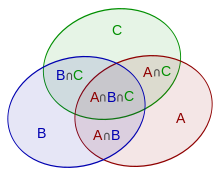
\includegraphics[width=0.2\linewidth]{img/venn-inclusion-exclusion}
	\label{fig:venn-inclusion-exclusion}
\end{figure}


Entonces el área de su unión $A \cup B \cup C$ es igual a la suma de las areas $A$, $B$ y $C$ menos áreas doblemente cubiertas $A \cap B$, $A \cap C$, $B \cap C$, pero con la adición del área cubierta por tres conjuntos $A \cap B \cap C$:

$$S(A \cup B \cup C) = S(A) + S(B) + S(C) - S(A \cap B) - S(A \cap C) - S(B \cap C) + S(A \cap B \cap C)$$

También se puede generalizar para una asociación de $n$ conjuntos

\subsection{La formulación en términos de la teoría de la probabilidad}

Si $A_i$ $(i = 1,2...n)$ son eventos y ${\cal P}(A_i)$ la probabilidad de un evento de $A_i$ de ocurrir, entonces la probabilidad de su unión (es decir, la probabilidad de que al menos uno de los eventos ocurra) es igual a:

\begin{eqnarray} 
	{\cal P} \left( \bigcup_{i=1}^n A_i \right) &=& \sum_{i=1}^n{\cal P}(A_i)\ - \sum_{1\leq i<j\leq n} {\cal P}(A_i \cap A_j)\ + \\ &+& \sum _{1\leq i<j<k\leq n}{\cal P}(A_i \cap A_j \cap A_k) - \cdots + (-1)^{n-1} {\cal P}( A_1 \cap \cdots \cap A_n ) 
\end{eqnarray}

Y de forma más compacta:


$${\cal P} \left(\bigcup_{i=1}^n A_i \right) = \sum_{\emptyset \neq J\subseteq \{1,2,\ldots,n\}} (-1)^ {|J|-1}\ {\cal P}{\Biggl (}\bigcap_{j\in J}A_{j}{\Biggr )}$$

Para la demostración es conveniente utilizar la formulación matemática en términos de teoría de conjuntos:

$$\left|\bigcup_{i=1}^n A_i \right| = \sum_{\emptyset \neq J\subseteq \{1,2,\ldots ,n\}} (-1)^{|J|-1}{\Biggl |}\bigcap_{j\in J}A_{j}{\Biggr |}$$

Queremos probar que cualquier elemento contenido en al menos uno de los conjuntos $A_i$ ocurrirá en la fórmula solo una vez (tenga en cuenta que los elementos que no están presentes en ninguno de los conjuntos $A_i$ nunca se considerará en la parte derecha de la fórmula).

Considere un elemento $x$ ocurriendo en $k \geq 1$ conjuntos $A_i$. Mostraremos que se cuenta solo una vez en la fórmula. Tenga en cuenta que:

\begin{itemize}
	\item en términos que $|J| = 1$, el objeto $x$ será contado $+\ k$ veces;
	\item en términos que $|J| = 2$, el objeto $x$ será contado $-\ \binom{k}{2}$ veces porque se 
	contará en aquellos términos que comprendan dos de los $k$ conjuntos que contienen $x$;
	\item en términos que $|J| = 3$, el objeto $x$ será contado $+\ \binom{k}{3}$ veces;
	\item $\cdots$
	\item en términos que $|J| = k$, el objeto $x$ será contado $(-1)^{k-1}\cdot\binom{k}{k}$ veces;
	\item en términos que $|J| > k$, el objeto $x$ se contará cero veces;
	
\end{itemize}

Esto nos lleva a la siguiente suma de coeficientes binomiales :

$$T = \binom{k}{1} - \binom{k}{2} + \binom{k}{3} - \cdots + (-1)^{i-1}\cdot \binom{k}{i} + \cdots + (-1)^{k-1}\cdot \binom{k}{k}$$

Esta expresión es muy similar a la expansión binomial de $(1 - x)^k$:

$$(1 - x)^k = \binom{k}{0} - \binom{k}{1} \cdot x + \binom{k}{2} \cdot x^2 - \binom{k}{3} \cdot x^3 + \cdots + (-1)^k\cdot \binom{k}{k} \cdot x^k$$

Cuando $x = 1$, $(1 - x)^k$ se parece mucho $T$. Sin embargo, la expresión tiene un adicional  $\binom{k}{0} = 1$, y se multiplica por $-1$. Eso nos lleva a $(1 - 1)^k = 1 - T$. Por lo tanto
$T = 1 - (1 - 1)^k = 1$, lo que se requería probar. El elemento se cuenta una sola vez.

\subsection{Generalización para calcular el número de elementos en exactamente $r$ conjuntos}

El principio de inclusión-exclusión se puede reescribir para calcular el número de elementos que están presentes en conjuntos cero:

$$\left|\bigcap_{i=1}^n \overline{A_i}\right|=\sum_{m=0}^n (-1)^m \sum_{|X|=m} \left|\bigcap_{i\in X} A_{i}\right|$$

Considere su generalización para calcular el número de elementos que están presentes en exactamente $r$ conjuntos:

$$\left|\bigcup_{|B|=r}\left[\bigcap_{i \in B} A_i \cap \bigcap_{j \not\in B} \overline{A_j}\right]\right|=\sum_{m=r}^n (-1)^{m-r}\dbinom{m}{r} \sum_{|X|=m} \left|\bigcap_{i \in X} A_{i}\right|$$

Para probar esta fórmula, considere algunos $B$. Debido al principio básico de inclusión-exclusión podemos decir al respecto que:

$$\left|\bigcap_{i \in B} A_i \cap \bigcap_{j \not \in B} \overline{A_j}\right|=\sum_{m=r}^{n} (-1)^{m-r} \sum_{\substack{|X|=m \newline B \subset X}}\left|\bigcap_{i\in X} A_{i}\right|$$

Los conjuntos del lado izquierdo no se intersecan por diferentes $B$, por lo que podemos resumirlos directamente. También se debe tener en cuenta que cualquier conjunto $X$ siempre tendrá coeficiente $(-1)^{m-r}$ si ocurre y ocurrirá exactamente $\dbinom{m}{r}$ conjuntos $B$ .